\documentclass[a4paper]{report}
\usepackage[utf8]{inputenc}
\usepackage[numbers]{natbib} % scientific references in the bibliography
\usepackage{hyperref}
\usepackage{graphicx}
%\usepackage{datetime}
\usepackage{color}
\usepackage{perpage} %the perpage package
\MakePerPage{footnote} %the perpage package command
%\usepackage{microtype}
%\usepackage{draftwatermark}
\usepackage{float}
\usepackage{listings}

\floatstyle{plain} % optionally change the style of the new float
\newfloat{Code}{H}{myc}

\lstset{literate=%
{å}{{\aa}}1
}
\lstset{extendedchars=\true}
\lstset{inputencoding=ansinew}


\newcommand{\todo}[1]{\footnote{{\color{red} TODO: #1}}}

% ------------------------------------------------------------------------------
% Metadata
% ------------------------------------------------------------------------------
\title{Ontology Learning from Swedish Text}

\author{Jan Daniel Bothma}

% ------------------------------------------------------------------------------
% Document
% ------------------------------------------------------------------------------
\begin{document}

\maketitle

\begin{abstract}
\end{abstract}	

\tableofcontents

\chapter{Introduction}
%ONE-SENT Ontology learning learning tools significantly speed up the knowledge extraction part of the Knowledge Engineering process. I'm going to investigate ontology learning from Swedish text.

%%UU-CHAP Motivation for the Project
%%UU-CHAP Background to the problem or system
%%"I am going to look at the following things"
Data collection and computer support for many tasks is prevalent.
Yet a large part of implementation of software support and combining several systems is still manual.
The precise meaning of data is often encoded directly in the software, which means that interpretation is repeatedly encoded in various systems using that data.
Software systems can help with smaller tasks, but the combination of various systems is again either done manually by the user, or the interpretation of the systems is encoded in more software.

By encoding semantic information about the world in a form that can be processed by computers, computers can provide better support in many tasks, with less manual and repeated definition of the meaning of the data being exchanged.
In a hypothetical example of this given in \todo{ref TBL semantic web 01}, a brother and sister try to schedule when they can drive their mother to medical facilities can treat her illness and is covered by her medical insurance.
Instead of manually gathering the data and doing the scheduling, the siblings give the problem to "agents", or computerised actors which together solve the problem using shared ontologies of treatments and facilities, insurance and scheduling, and data from all the parties anotated with relationships to those ontologies.

The task of annotating data with semantics and building the ontologies that define it is a time-consuming process.
Domain experts are needed to accurately describe the important semantics of each domain.
Ontology engineers are needed to concisely encode these semantics in a manner that is useful for automated reasoning.
Mistakes in defining ontologies can result in ontologies from which incorrect or insufficient conclusions are drawn, and can make it difficult to maintain the ontology.

One approach to reduce the demands on domain experts and ontology engineers is ontology learning.
Ontology learning aims to automatically or semi-automatically construct ontologies, with little or no supervision.
Ontology learning from text specifically does this from natural language text.
This is an important area of research because much of the knowledge that would be useful if encoded in ontologies, is already recorded in text documents, for example business memoranda and communication, and scientific papers.

Ontology learning from text tends to employ a variety of natural language processing techniques to identify syntactic features in the text, then use stastical and linguistics-based methods for extracting evidence of concepts of the domain, and their relationships and properties.
Some systems attempt to automatically construct ontologies in formats ready for application in semantically-enabled software, while others present the evidence as an aid to human experts who can then build such ontologies with significantly-reduced effort compared to a manual approach.

\section{Problem}
%ONE-SENT Hoewever, there is no Ontology Learning System for learning ontologies from Swedish text.

Most ontology learning research forcuses on English language.
This research is showing useful results and has been applied successfully in various projects, however none of these systems currently support ontology learning from Swedish text.
There appears to be no ontology learning software system that has been applied to learn ontologies from Swedish text.
\todo{Hjelm's thesis\cite{Hjelm09Thesis} learnt a "prototypal" ontology from several languages including swedish.
We can learn a bit from it, but he used terms from an existing ontology, and we need to check if the relations they learnt are applicable.}
While most scientific research in Sweden is now published in English and many businesses are using English internally, there is still a wealth of existing and new literature from the business and scientific domain which would be valuable in semantically-enabled software.
The problem is therefore that ontology learning should be extended to support Swedish text, making use of existing research in natural language processing and information extraction for Swedish where necessary.
 
\section{Objective}

The objective of this thesis is to develop a system for ontology learning from Swedish text.
Given the time constraint, only a prototype will be built which will apply a small selection of methods, with the objectives of
\begin{enumerate}
  \item Suggesting concepts and relations for building a domain ontology given a corpus of domain text
  \item Supporting the semi-automatic constuction of such an ontology
  \item Identifying issues for the further development of such a system
\end{enumerate}

\section{Delimitations}

The restriction to a small selection of methods means that only certain kinds of concepts and relations can be extracted and important things might be missed.
This is because certain methods are only suited to particular syntactic or semantic forms.

The construction of an ontology usually needs to take the end application of the ontology into account.
For example, decisions about which relations should be included, or whether a term is a general concept or a concrete instance, usually depend on the intended application.
We do not want to favour a particular application and do not make providing such flexibility an explicit objective for this prototype, but will instead attempt to produce a general representation of the domain.

\todo{not sure if the following is relevant to this section but leaving here for now.}
it'd be nice but I probably won't be able to ground my ontologies in any upper ontologies (ontology matching and ontological architecture).
Maybe this is easy or critical and I can revise this entry.

There's a lot of research into using internet phenomena like croud sourced data and stuff.
We're focusing in extracting information from any Swedish text.
This means we can produce results for domains that have very little or unrepresentative data online (but depends on finding some representative corpus).
These approaches also have issues like access to the services and reliability of the data.
For these reasons, we're not trying the web-sourced stuff specifically.

\section{Research Questions}

To fulfill this objective, this report attempts to answer the following research question:

\begin{enumerate}
	\item How can Swedish Text be used for semi-automatically constructing domain ontologies?
\end{enumerate}

\section{Approach}
%ONE-SENT

This section needs to identify and show how we avoid possible sources of bias.

The basis of our method is how OL has been applied to other comparable languages like German with its compounding, and what's been learnt from the existing work on information extraction from Swedish.

The implementation should probably be based on the architecture proposed in \cite{Cimiano2009OL}

NLP tools for the common annotations are available and under further development, partly as a result of the BLARK for Swedish project.

The procedure is something like set up preprocessing, apply existing methods to swedish, evaluate, tweak for swedish, evaluate.

Ideally we can repeat an experiment for English and reproduce their results, to support the assertion that our implementation is ok.

I think I'll evaluate taxonomy extraction against the Eurovoc thesaurus since I can probably get hold of corpora for one or more of the topics they cover.

The implementation will probably be integrated with some OE system.
Protege 4+ looks nice since it has decent, modern libraries and tools and plugin framework.



\section{Report Structure}

\chapter{Background}
%%UU-CHAP Overview of relevant research and development that is used in specifying the problem and obtaining and evaluating appropriate solutions.
%%ONE-SENT Many methods for the subtasks have been developed for other languages, and some have already been applied to Swedish, but they have not been combined and evaluated as a pipeline. Furthermore, none of the existing OL systems are suitable to be extended to Swedish, nor support the necessary evaluation approaches.
%%UU-REQ Awareness of relevant prior research and development literature
%% -- comment on its relevance. In what way _is_ it relevant and in what way is it _not_ relevant.
%%UU-REQ critical appraisal of that literature as a basis for the formulation of project objectives and the conduct of the project.
%% -- quality of the literature affects its bearing on the project. Note on the quality of an evaluation keeping in mind whether a plain olde eval would have been suitable in the first place - what's the objective of the publication?

This chapter gives an overview of the theoretical background to this thesis.
The relationships between Ontology Learning from Text and its surrounding disciplines are identified in Sec.\ref{sec:lit-rev:parents}, then work and issues relevant to this field and this thesis specifically are discussed in Sec.\ref{sec:lit-rev:immediate}.

\section{Parent disciplines}
\label{sec:lit-rev:parents}

This section identifies the relationships between Ontology Learning from Text, and the surrounding disciplines.
At a high level, Knowledge Management and the Semantic Web form the basis of applications that are supported by semantics encoded in a manner that allows automated reasoning.
Ontology Learning is related with Knowledge Acquisition and Representation as a specific form of these processes, and the relation between Machine Reading and Ontology Learning is covered briefly.
Some of the parts Ontology Learning plays in Ontology Engineering are identified, and finally the broader field of Ontology Learning is described, leading to a definition of Ontology Learning from Text.

\begin{figure}
  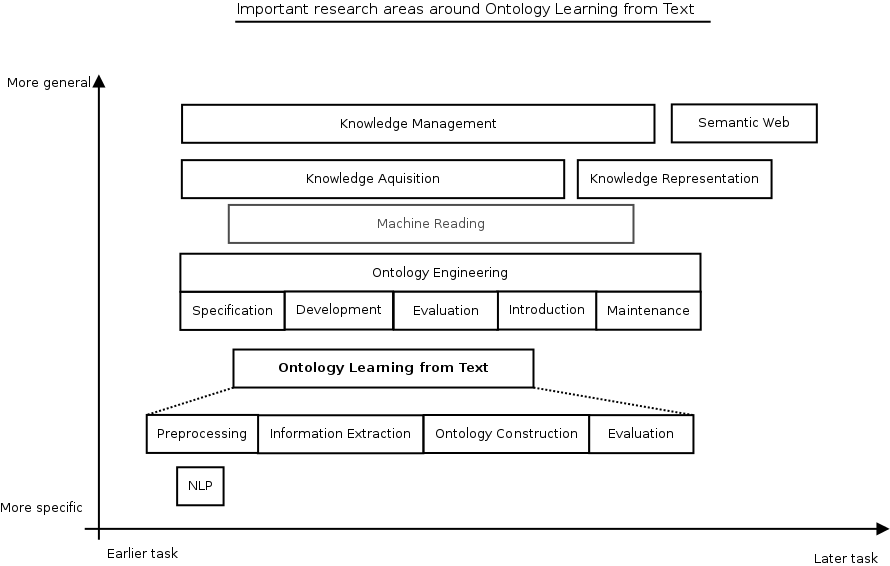
\includegraphics[width=\textwidth]{graphics/related-research-fields.png}
  \caption{Related research fields}
  \label{fig:related-research}
\end{figure}



\subsection{Knowledge Management}

Knowledge Management involves creation, storage, retrieval, transfer and application of the tacit and explicit knowledge pertaining to an organisation \citep{AlaviLeidner2001KM}.
Knowledge has been shown to be a significant asset in organisations, and information technology can help making such knowledge available to areas where the knowledge is not transferred easily \citep{AlaviLeidner2001KM}.

An example of using information technology to collect, store and apply valuable organisational knowledge is the \emph{semantically enabled} IURISERVICE iFAQ database of legal questions and answers given by experienced Spanish judges.
This tool aims to support inexperienced judges in answering legal questions\cite{IURISERVICEPerformance2007}.
Important terms in the questions and answers are associated with their synonyms and the domain of law that they apply to.
When a question is entered to search for related question-answer pairs, the semantic information is used to improve the results over a plain text search, even when considering different forms of the words in the query.
The query is expanded to include exact matches, morphological variations\footnote{In the linguistic sense, such as \emph{car} to \emph{cars} for plurality}, and synonyms.
The similarity of the result questions to the query question is then calculated, considering the similarity of concepts and the grammatical structure of the questions, to provide the most-similar results to the user.
The semantic information is further used to provide suggestions of relevant legal cases whose decisions might have an impact on the issue at hand.

\subsection{Semantic Web}

By making semantically annotated information available over the internet, many resources can be combined to support complex tasks involving many parties.
The Semantic Web\footnote{http://www.w3.org/2001/sw/} is the manifestation of this.
In a hypothetical example, Tim Berners-Lee et al. \footnote{Tim Berners-Lee, James Hendler and Ora Lassila. The Semantic Web. \emph{Scientific American}, 284(August), 2001} describe a scenario where a brother and a sister try to book medical appointments for their mother with a nearby treatment centre available to their mother's health insurance policy, on dates that they can alternate driving their mother.
Information about their availability, the clinics (including treatments they offer and their schedules) and the insurance policy must be available to the computers involved in proposing a solution.
Furthermore, the meaning of this information, and how it relates to the other information involved in the computation, must be available.
For example, the computer must be able to distinguish between the treatment centre's postal address and their visiting address.
This information is encoded in ontologies and mappings between semantic entities in standardised formats such as OWL\cite{OWLOverview2004} to support this interoperability.

The masses of information available as plain text is not directly usable in the semantic web.
Knowledge must be encoded in machine-readable forms compatible with the Semantic Web.
That knowledge can come from a variety of sources, and the process of gathering knowledge for storage and application in semantically-enabled systems is known as Knowledge Acquisition.

\subsection{Knowledge Acquisition}

Knowledge Acquisition in the context of information technology is the elicitation and interpretation of knowledge about a particular domain for use in knowledge-based systems \citep{anjewierden1987KATools}.
This corresponds to the acquisition part of Knowledge Management and is a precursor to Knowledge Representation. 

\subsection{Knowledge Representation}

Knowledge Representation is the discipline of encoding knowledge in a form that facilitates computer inference based on that knowledge, drawing conclusions not explicitly present in already.
In this thesis we focus on ontology-based knowledge representation.

\subsection{Ontologies}
\label{sec:lit-rev:ontologies}

A commonly-cited definition of ontologies in the field of knowledge engineering is as \emph{``a formal, explicit specification of a shared conceptualization''} \cite{StuderEtAl1998KEPM}.
Here, a \emph{conceptualization} is the objects, concepts and relations between them, in an abstract view of the world intended for a particular purpose.
The conceptualization should be \emph{shared} within the context of its application.
The objective with this explicit specification is to allow computer agents to operate on this view of the world or for its integration in human-operated software.

Ontologies that represent a particular domain are known as \emph{Domain Ontologies}.
One way to support integration of several domain ontologies is by defining elements common to many domains in an \emph{upper ontology}\cite{SemanticIntegration2004Noy}.

\todo{could distinguish between "lexical" and non-lexical ontologies like what Hjelm and I think Cimiano refers to.}

In this thesis we focus on description logic ontologies, and in particular on OWL, the Web Ontology Language.

\subsection{Ontology Engineering}

The discipline of specifying, developing, introducing and maintaining ontologies for some application is known as \emph{Ontology Engineering} (OE)\cite{HOO2009OntEngMeth}.
Along with broader considerations of OE such as the intended users and software engineering issues, the domain expert(s) and ontology engineer must gather relevant domain knowledge (Knowledge Acquisition) and encode it in a computer-readable form (Knowledge Representation)\cite{OntMethOverv1999}.
This is challenging and repetitive and is known as the Knowledge Acquisition Bottleneck\cite{OLforSemWeb2001}.
As an example, a "tasks and skills" ontology in the case study in \cite{HOO2009OntEngMeth} consisted of about 700 concepts after refinement.
Automating as much as possible of the knowledge acquisition and representation can reduce the effort for domain experts and ontology engineers when developing and maintaining ontologies\todo{need to back this up}.

\subsection{Ontology Learning}
\label{sec:background:ontlearning}

The automatic or semi-automatic construction of ontologies from domain data is called Ontology Learning \cite{Cimiano06}.
Ontology Learning (OL) can start with structured, semi-structured or unstructured data as input \cite{Cimiano2009OL}.
Structured data, such as databases, can be somewhat independent of language and its semantics are described by its schema or structure \todo{I think \cite{Cimiano2009OL} is sufficient but need to check}.
Most methods for ontology learning from semi-structured data such as wikis and unstructured data in the form of plain text depend on preprocessing techniques from the field of Natural Language Processing (NLP) to provide syntactic annotations like part of speech or syntactic dependencies.
OL methods are then applied to the annotated corpus, each method extracting one or more kind of ontology element.

Ontology learning software systems have been implemented that provide one or more algorithms for extracting concepts, relations and axioms from a text corpus.
Such systems are often integrated with dedicated NLP tools to provide the required preprocessing facilities.
Extracted elements are manually or automatically added to an ontology and can often be output in a standard ontology serialisation format like OWL\cite{OWLOverview2004}.

Ontology learning methods have varying degrees of language dependence.
In the simplest case, an OL system can be applied to another natural language by replacing the language models in the NLP components with models trained on the other language.
However, often the syntactic and semantic structure of languages vary enough to require modifications to OL methods or the process as a whole \cite{Voelkner2008Spanish}\todo{saying "often" probably means we need more than one example}.

\subsection{Ontology Learning from Text}
\label{sec:background:ontlearning-text}

This section defines Ontology Learning from text and discusses important work in this field.
More detail of the tasks and methods of Ontology Learning from Text is covered in Sec.\ref{sec:lit-rev:immediate}

Ontology Learning from Text is the process of building a formal ontology from a semi-structured or unstructured text corpus from a particular domain \citep[p.3-7]{Cimiano06}.
The ontology is intended to model the concepts and the semantic relationships between the concepts in the domain.
Ontologies are further described in Sec.\ref{sec:lit-rev:ontologies}.

The typical tasks and their outputs are shown in Fig.\ref{fig:output-task-technique}.

\begin{figure}
  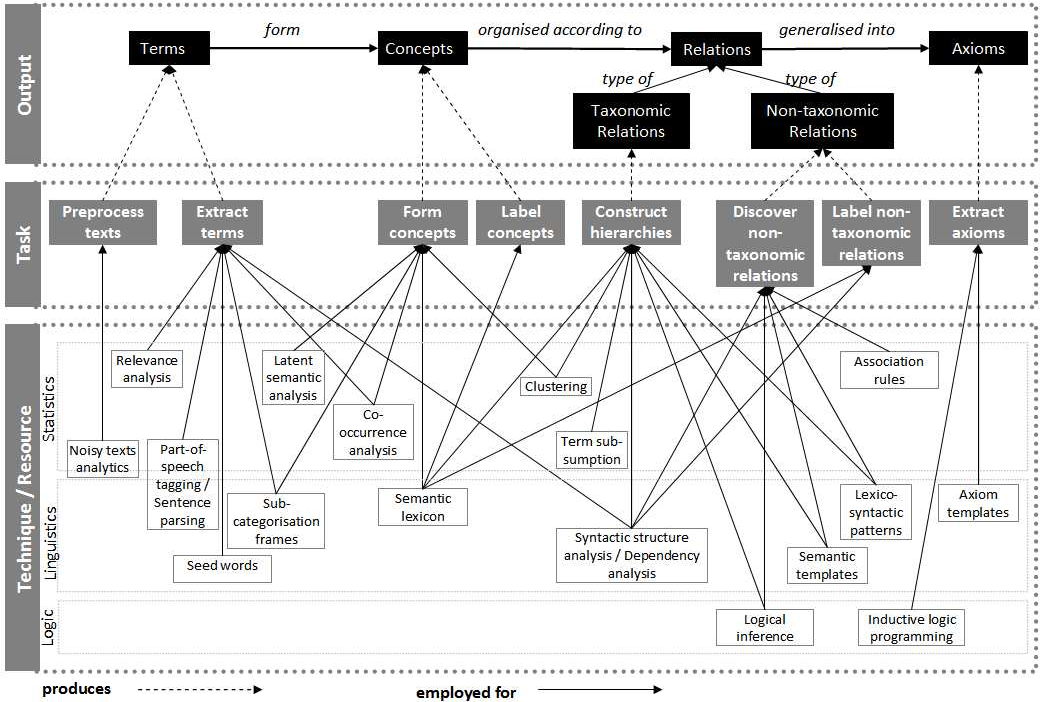
\includegraphics[width=\textwidth]{graphics/output-task-technique-WongLiuBennamoun.png}
  \caption{Tasks, techniques and outputs in ontology learning. \cite{Wong2009PhD}}
  \label{fig:output-task-technique}
\end{figure}


\subsection{Machine Reading}

Machine Reading is the automatic, unsupervised \emph{'understanding'} of text where understanding means formation of beliefs supporting some level of reasoning from a textual corpus \citep{EtzioniEtAll06MachineReading}.
Machine Reading is distinguished from Information Retrieval where this is done in a in a highly supervised, manual manner - for example where patterns for extracting desired entities are hand-written or manually selected from an extracted list.
Machine reading strives instead for extracting arbitrary semantic relations without human supervision \citep{EtzioniEtAll06MachineReading}.

While Cimiano concluded that some level of supervision is necessary in Ontology Learning from Text \citep{Cimiano06}, recent work in Ontology Learning from Text such as OntoUSP\citep{Poon2010OntoUSP} and OntoCMaps \citep{Zouaq11OntoCmaps} shows progress towards learning arbitrary relations with high precision and recall in an unsupervised manner, which is much closer to machine reading than earlier work in the field.


\section{Immediate discipline}
\label{sec:lit-rev:immediate}

This section describes relevant research in ontology learning from text.
The descriptions are organised according to the role the research plays within the field and its processes.

The key issues for ontology learning from text are shown in \ref{fig:ol-issues}.
OL from text starts with collecting and preparing text corpora.
The corpora must be preprocessed as needed by the information extraction methods.
Evidence for potential ontology elements might be combined from various methods with overlapping scope.
An ontology is constructed using the extracted information, which is generally evaluated during or following construction.
As with ontology engineering, change management and user interaction are important aspects throughout the process.

Methods were chosen for inclusion in this review based on their relevance to this thesis and research in general.
While ontology learning from text includes extraction from structured text, this thesis avoids the specificity of methods for structured data.
Domain independent methods are preferred over domain-specific such as \cite{LeeEtAl03OLMed} for medicine.
Methods depending heavily on existing knowledge bases are avoided such as \cite{Gulla08LOUIE} for its dependence on film knowledge bases or \cite{Drumond10PREHE} and \cite{HaiTaoEtAl08Clonto} for dependence on WordNet\cite{Fellbaum98WordNet}.
While general domain knowledge bases such as WordNet and Cyc\cite{Lenat95Cyc} can help extract so-called \emph{low hanging fruit} and there even exists a WordNet for Swedish\cite{Viberg02SWordNet}, it generally takes a lot of effort to extend such databases to a new domain \footnote{This is in fact closely related to OL for domain ontologies} and they might introduce errors since the senses of words and phrases in specific domains might be different from those in general language.
Their consideration is left for further research.

\begin{figure}
  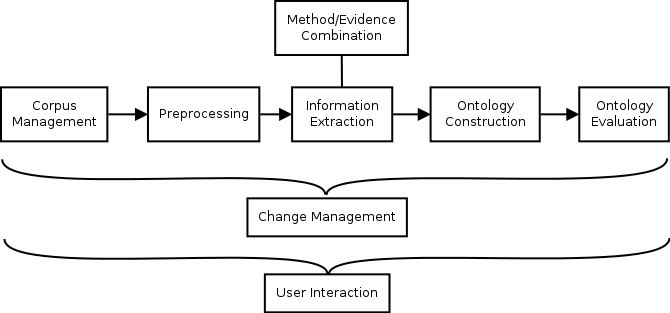
\includegraphics[width=\textwidth]{graphics/ontology-learning-system-issues.png}
  \caption{Issues for Ontology Learning systems}
  \label{fig:ol-issues}
\end{figure}

\subsection{Ontology Learning Tasks}

Ontology learning is typically defined in terms of several tasks, namely Preprocessing, Term Extraction, Concept Extraction, Relation Extraction, Axiom Extraction, Ontology Construction and Evaluation.
Later tasks tend to build upon the earlier tasks, although tasks are carried out in parallel or revisted in various methods.
Task definitions are mainly useful for defining the scope of a given part of the ontology learning process.

In figure~\ref{fig:ol-issues} I combined Term, Concept, Relation and Axiom extraction under the issue of Information Extraction.
I further added Corpus Management; Method and Evidence Combination; Change Management and User Interaction as \emph{issues} of interest in a slightly higher level view of the Ontology Learning process.
These areas are defined below with the aim of defining the scope of the work in this thesis and the extent to which each issue is given attention here.

\subsection{Corpus Management}

Corpus management involves selection of suitable corpora and storage of changes and annotations made during Preprocessing and Information Extraction.
A corpus is a collection of documents compiled for linguistic investigation or processing \citep{KokkinakisGerdin10MedCorp}.
When performing ontology learning from text, a corpus must be compiled which contains the text from which the domain model must be extracted.
Selection of suitable corpora is important since the authority of the derived ontology depends on the authority and relevance of the source text for the domain.
Annotations are generally made by NLP tools to identify linguistic features of text such as parts of speech or syntactic dependencies.
These features are then used by one or more information extraction techniques.

Maintaining the annotations of these features in the context they occur in, as opposed to simply extracting fragments and their features to a database, is necessary for some information extraction methods\citep{Frantzi98CNCValue, NenadicEtAl02TermSim, Srikant95GenAssocRul} and helps with ontology learning evaluation and research.

Many annotation formats exist including XML, other plain text formats and more complex binary formats.
Various NLP tools such as the Stanford parser \citep{Marneffe06StanfPars} and FM-SBLEX morphology tools support input and output in XML and several other formats for different applications.
A common plain text annotation format consists of one token string and its corresponding annotation on the same line, with only one token per line.
This format is output by the HunPos tagger, for example, and can be accepted as input by MaltParser\citep{Nivre06maltparser} and FM-SBLEX.
XML facilitates programmatic transformation and processing, although the XML schemas vary significantly meaning tools are often not directly compatible.
For example, the XML formats of the Genia corpus \citep{KimEtAl03GeniaCorpus}, the FM-SBLEX tools and the Stanford NLP tools are significantly different.\todo{Add CoNLL format\citep{NivreEtAl07NoNLL} used by \citep{Nivre06maltparser}}.

Existing corpora and common document formats often already contain features and annotations that can be useful in ontology learning.
For example, section headings can be extracted from HTML, PDF and Word documents, and coreferences (See Sec.\ref{sec:lit-rev:preproc}) are identified using XML in the Genia corpus.
GATE can accept a variety of input document formats and normalises the structure of non-plain-text formats like HTML, Microsoft Word documents and PDF to its internal annotation format with common labels for annotation types among all normalised input formats \citep{Cunningham2011GATEBook}.
The Korp annotation pipeline can accept various XML formats, and strip, copy or ignore and in some cases use existing annotations \cite{Borin12Korp}.

The multitude of annotation formats forming input and output of the numerous tools creates a challenge for corpus management.
GATE helps deal with this challenge with over ten years of refinement.
The GATE Developer application provides user interfaces to review and edit annotations manually, while the GATE Embedded Java libraries can be used programmatically to integrate various NLP tools during preprocessing and annotation.
References to annotations can be stored by external applications to retrieve annotations for the change management tasks.

\subsection{Preprocessing}
\label{sec:lit-rev:preproc}

Preprocessing is the task of ensuring the corpus is in a suitable state for the information extraction methods to be effective, and annotating the corpus with linguistic features needed by certain information extraction methods.
Common preprocessing tasks for ontology learning include
\begin{itemize}
  \item tokenisation
  \item sentence splitting
  \item part of speech and morphology analysis
  \item lemmatisation or stemming
  \item named entity recognition
  \item coreference resolution
  \item chunking
  \item syntactic dependency parsing
\end{itemize}
An additional task of \emph{compound splitting} is important for languages where compound words are common without a separating space or hyphen, such as Swedish, German or Russian.

\subsubsection{Tokenisation}

Tokenisation identifies individual word units - mainly separated by spaces but possibly also punctuation characters.
Many NLP methods operate on individual tokens in the corpus.
For example, a part of speech tagger assigns a part of speech to individual tokens, perhaps taking the sentence context into account.
In certain domains word units might include characters that would be classed as token separators in common natural language.
Generic tokenisation methods might need modification when performing ontology learning on such domains.

\subsubsection{Sentence splitting}

Sentence splitting identifies individual sentences - sometimes taking document layout into account to improve accuracy when full-stops are missing, in headings, for example.

\subsubsection{Part of speech and morphology analysis}

Part of speech tagging, or POS-tagging, assigns grammatical word categories to individual words or other tokens such as numbers.
A tagset defines how certain features are represented.
For example in the Penn Treebank tagset, a singular common noun is tagged NN, while a plural common noun is tagged NNS \citep{Marcus93Penn}.
Tagsets often include morphosyntactic categories such as gender, number and case.

Two interchangeable tagsets are commonly used for swedish: the PAROLE tagset and the SUC tagset \citep{Forsbom08Tagging}.
A mapping is available between these tagsets \footnote{http://spraakbanken.gu.se/parole/tags.phtml}.
These tagsets support common morphosyntactic categories, for example a common singular indefinite noun of neuter gender in the nominative case such as \emph{raketvapen} (english \emph{missile}) would have the tag {\tt NCNPN@IS} in the PAROLE tagset and {\tt NN NEU PLU IND NOM} in the SUC tagset.

Many taggers are available, and they can often be configured to use custom language models.
Such language models are specific to the language being tagged and are usually generated from a treebank - a corpus with annotations produced with high-enough accuracy to be used as training data for building language models and performing linguistics research.
Models for tagging Swedish text are available from Eva Forsbom \footnote{http://stp.lingfil.uu.se/~evafo/resources/taggermodels/models.html} and Beata Megyesi \footnote{http://stp.lingfil.uu.se/~bea/resources/} and embedded in the Korp pipeline. \todo{maybe something about tagger accuracy, some literature, this is lit-rev after all}

\subsubsection{Lemmatisation and stemming}

Lemmatisation and stemming both attempt to normalise words from their inflected forms to some common form.
Stemming removes common prefixes and suffixes, leaving the 'stem' behind which may not be a word in the language, for example changing \emph{kloster} and \emph{klostret} (\emph{monastery} and \emph{the monastery} respectively) to \emph{klost}.
Lemmatisation modifies words to their lemma, or uninflected form, changing \emph{klostret} to \emph{kloster} and leaving \emph{kloster} as it is.

Lemmatisation is preferred in ontology learning since it is useful to distinguish different senses of a word while coalescing different inflections of the same sense.
Stemming is usually quite a course, rule-based approach which can lose important parts of words that look like pre- or suffixes but are part of the lemma \todo{ought to cite this, \citep{Gacitua08OntoLancs} says \citep{Alkula01MeaningWords} deals with this.}, meaning many more senses of the same word would be coalesced than with lemmatisation.
The Saldo lexicon \cite{Borin09Saldo} goes a step further, by assigning unique identifiers based on the lemma to distinguish between different senses of words with the same lemma.

When lemmatising words, the appropriate sense of the word must be chosen to select the correct lemma.
Unsupervised preprocessing means that a native speaker is not available to identify the sense of the word by its meaning.
The Korp pipeline attempts to improve sense selection by choosing the sense with the most-similar morphology, such that a noun would be chosen over a verb given a word tagged as a noun, for example.

The FM-SBLEX word analysis tools and the Korp pipeline are based on the Saldo lexicon.
The FM-SBLEX tool can lemmatise words not in the lexicon, such as \emph{kommunerna} (english \emph{the municipalities}).


\subsubsection{Named Entity Recognition}

Named Entity Recognition is the identification of instances of real world entities such as persons or organisations, referenced by name in the corpus.
This is useful, for example, for identifying attributes and relations of these instances or their classes.

\subsubsection{Coreference Resolution}

Coreference Resolution associates multiple references to the same instance with each other.
For example, in the sentence "John ate the apple that he picked up", John and he would be identified as references to the same instance.
This helps deal with data sparseness.
Without coreference resolution, only full references using the full term, are accurately identified as occurences of the concept as itself and as part of relations.

\subsubsection{Chunking}

Chunking, or shallow parsing, identifies non-overlapping parts of sentences playing various roles in the sentence, for example identifying the noun phrases making the subject and object parts in the sentence.
The SweSPARK chunker employs a parser for chunking Swedish text \cite{Megyesi02Thesis}.

\subsubsection{Syntactic Dependency Parsing}

Syntactic dependency analysis produces a dependecy graph where the vertices are the words in a sentence and an edge exists between each word and its syntactic head.
The graph forms a tree rooted at the main verb.
The edges can be labeled with dependency types.

Syntactic dependencies are often used for extracting labeled relations between terms, and for determining the selectional restriction of the arguments to verbs.
The OntoUSP \citep{Poon2010OntoUSP} method and the methods in the OntoCMaps system \citep{Zouaq11OntoCmaps} make use of syntactic dependencies for identifying roles of phrases in the corpus, leading to labeled relations.

\subsubsection{Compound Splitting}

FM-SBLEX provides compound analysis, giving sets of two or more word senses from its lexicon that might have been compounded to form the word in question.

The relation extraction method in \cite{Kokkinakis08SolidComp} used a glossary of domain terms to select likely compound parts from the possible part pairs.

A statistical model of the swedish language is used in \citep{Sjobergh04Compounds} to split compounds. This was used for the Swedish compund splitting in \citep{Hjelm09Thesis}.

\subsubsection{The SVENSK language processing toolbox for Swedish}

SVENSK is a language processing toolbox for Swedish developed in the late 1990s and 2000\cite{OlssonGamback00SVENSK}. SVENSK aimed to support research and teaching which depended on Swedish language processing by providing common text processing tools such as taggers and parsers in a general purpose language processing framework. SVENSK was based on the GATE language processing framework.

\subsection{Information Extraction}

Information Extraction is the task of extracting structured information from a corpus of text.
The units of information generally extracted are terms, concepts, attributes, relations and axioms.
The approaches for extracting knowledge from the preprocessed corpus are usually based primarily on statistics, linguistings or logic.

\subsubsection{Terms, Concepts and Instances}

Terms are common lexical references to concepts within a domain.
In this context, \emph{instances} are specific instances of concepts.
For example, \emph{book} is the term for the concept of a collection of paper bound together, and the copy of \todo{cite noun phrase book} on my book shelf is an instance of a book.
It is in fact an instance of the named entity \emph{Feature Distribution in Swedish Noun Phrases}, a subclass of book.

The precise distinction between concept and instance depends on the requirements of the application - the level of abstraction varies depending on exactly what is being modeled and how it needs to be interpreted.
When building ontologies, concepts are elements of the ontology which models the domain, while instances populate the ontology and their meaning are defined by the ontology.

The distinction between concept and term becomes more important towards the formal end of the scale of knowledge representation.
The less-formal levels like taxonomies and thesauri are based on terms.
On the other hand, the definition a formal ontology and its use in reasoning is based on unique references to concepts, relations and axioms - a term is merely a human-readable label associated with such a reference.

Terms extraction tends to focus on noun phrases, although any lexical form used to refer to relevant concepts is important.
Common approaches define a way to select potential candidate terms, and then use some approach of ranking and selecting important terms from those extracted from the corpus.
Lexico-syntactic patterns on part of speech annotations, and particular subtrees of syntactic dependency trees are common ways of selecting candidate terms.
The TF-IDF and C/NC-value approaches are well-established statistical ways of ranking terms based on their occurence in the corpus, while a common alternative approach is to select terms based on the importance of the relations to which they are arguments.

The C-Value part of the C-Value/NC-Value method is used in this project.
This is a method for extracting multi-word terms from a domain corpus, assigning a numeric value to each candidate string, where a high value indicates important candidates - probable terms important to the domain.
Candidate strings can, for example, be selected via some lexico-syntactic pattern such as NounNoun+ (a series of two or more adjacent nouns) or Adj*Noun+ (zero or more adjectives followed by one or more nouns).
The frequency of occurrence of a candidate string contributes positively to C-Value.
The number of words in a candidate string contributes by its logarithm.
The occurrence of a candidate string nested in longer candidate strings contributes negatively to its C-Value.
The occurence of nested candidates within a candidate contributes negatively to the C-Value of that candidate.
These factors encourage longer candidates over shorter ones with the reasoning that longer terms are more specific and thus occur less frequently, and aren't represented fairly by frequency alone.
Meanwhile nested terms may be more general than terms containing them, or may they may not be terms by themselves at all.
Candidates which occur frequently within longer candidates but never by themselves are thus discouraged.

\subsubsection{Attributes and Relations}

Relations define the interactions between, and attributes of concepts.
A concept \emph{ball} might have the attribute \emph{colour}, where an intance of the ball has the color \emph{blue}.
Relations are typically classified as taxonomic or non-taxonomic.
Taxonomic relations include equivalence and hypynomy.
In the ball example, ball could be said to be a hyponym of sports equipment in a sports domain, while blue \emph{is a} colour.

Non-taxonomic relations then represent other interactions between concepts.
This can include merynomy - part-of relations - as well as representing how one concept can act upon another in the given domain.
Continuing the ball example, a player can kick a ball.
The \emph{kicks} relation might represent that players kick balls and not vice versa.
The player's foot is \emph{part of} the player, ie a meronym of the player.

In addition to identifying relationship between concept, some relationships also need extra work to assign a label to represent the semtantic relationship it represents.
Some approaches to relation learning stem from the label's occurrence in the corpus, like the \emph{kicks} relation above.
Others might merely be identified by some correlation of the concepts' occurrence in the corpus.
The difficulty in automating the labelling task means it is sometimes left to domain experts to do manually.

\medskip
Common approaches to extracting taxonomic relations are \emph{lexico-syntactic patterns}, \emph{agglomerative hierarchical clustering}, \emph{distributional similarity} and \emph{formal concept analysis} (FCA).

{\bfseries Lexico-syntactic patterns} define a pattern on lexical annotations on a corpus which are likely to represent intances of particular relations.
An example of such a pattern for English is $NP_{super}\ such\ as\ ((NP_{sub}, )* (NP_{sub}\ and))* NP_{sub}$.
Given a sentence ``Racquet sports such as squash, tennis and badminton are highly challenging", the above pattern would identify squash, tennis and badminton as subclasses of the concept \emph{racquet sport}.
Lexico-syntactic pattern tend to give high precision but low recall because of the variety of ways these relations can be expressed in natural language.
Variou approaches for mining these patterns have been developed.

{\bfseries Agglomerative Hierarchical Clustering} of concepts builds a hierarchy of clusters, starting with each concept as a distinct cluster.
Each clustering step compares each pair of clusters according to some \emph{similarity measure}, and the pair with the highest similarity are merged.
This repeats until some predicate is satisfied, for example when all clusters have been merged into one.
The initial clusters represent the most specific clusters, while the final cluster(s) represent the most general clustering.
If a clustering represents a concept, its more specific clusters might represent its subclasses.

{\bfseries Distributional Similarity} in its simplest form asserts that there exists a relationship between concepts which occur within some bounded context.
The strength of the relationship depends on the frequency of their co-occurrence.
The bounded context can for example be defined as the same document, a window of $n$ adjacent words in the corpus or as part of some subtree of a syntactic dependency graph.
The nature of the relationship can be inferred by how the concepts co-occur.
For example, if concept $A$ only occurs in the presence of concept $B$, and concept $B$ occurs more frequently than concept $A$, we might infer that $A$ and $B$ are related and that $B$ is more general than $A$.

{\bfseries Formal Concept Analysis} 
FCA considers the attributes which apply to each concept.
By analysing the attributes concepts share, a lattice of commonality and subsumption can be constructed.

\medskip

Non-taxonomic relation extraction approaches generally either extract relations where a concept is an argument to the main verb, or try to find some other association between a pair of concepts.

Verb-based approaches usually select candidates based on patterns defined on chunked sentences or paths in syntactic dependency trees.
These patterns and paths are often manually defined but may also be extracted by machine learning techniques.
The types of arguments accepted or required by a verb is known as its \emph{subcategorisation frame}.
The \emph{selectional restriction} of the verb is the instances of words that are valid arguments to the verb.
By identifying concepts which cover the selectional restriction of relations, the relation can be generlised at a convenient level.
The importance of the extracted relations in the domain is then determined using approaches based on statistical analysis, machine learning or graph theory, for example.

Other associations between concepts are often extracted based on shared features or occurrence in common contexts.
A common technique for this is based on \emph{association rule mining}.
This technique extracts rules indicating for a certain confidence value, which items occur only given the presence of others, or which items predict the presence of others.

\subsubsection{Axioms}

\todo{should probably include TextRunner/ReVerb since \cite{Poon2010OntoUSP} says its the state of the art in IE. At least the ReVerb website only mentions English}

\subsubsection{Semantics from Syntactic Dependencies}

I've avoided frames, but very relevant is \cite{JohanssonEtAl12RoleFrame} which builds a classifier using syntactic dependency relations as features to identify "semantic roles" for Swedish Framenet frames.
For example, the sentence "Vi promenerar s\"{o}derut..." has promenerar as frame SELF\_MOTION and subject Vi as SELF\_MOVER.
\todo{I should probably mention frames somewhere and explain why I've avoided it.
  One good reason is that swedish frames so far exist only for the general domain, medical domain and art domain\cite{JohanssonEtAl12RoleFrame}.}
This is similar to OntoUSP mapping dependency relations to different parts of horn clauses and OntoCmaps mapping dependency relations to "linguistic triple" relation parts.

\subsubsection{Method / Evidence Combination}

\subsection{Ontology Construction}

\subsection{Ontology Evaluation}
\label{sec:background:eval}
Ontology evaluation generally has two main purposes: for selecting the most appropriate existing ontology for an application; and for evaluating the performance of an instance of ontology engineering.
The latter is the objective when ontology evaluation is performed as part of ontology learning.

Eight main quality criteria for ontology learning are identified from the literature in \cite{HOO2009OntEval}, summarised here as short questions:

\begin{description}
\item [Accuracy] Does the ontology accurately model the domain?
\item [Adaptability] Can the ontology easily be adapted to various uses?
\item [Clarity] Is the meaning implied by the ontology clear?
\item [Completeness] Does the ontology richly or thoroughly cover the domain?
\item [Computational efficiency] How easily can automatic reasoners perform typical tasks?
\item [Conciseness] Does the ontology include unnecessary axioms or assumptions?
\item [Consistency] Does the ontology lead to logical errors or contradictions?
\item [Organisational fitness] Is the ontology easily deployed in the application context in question?
\end{description}

It is noted in \cite{HOO2009OntEval} that not all criteria are applicable in every case, and should be chosen and interpreted according to the requirements of each case.
Some might even be contradictory, for example completeness might work against conciseness\cite{HOO2009OntEval}.
This thesis is mainly interested in evaluating accuracy and completeness, as discussed in section~\ref{sec:methods:evaluation}.
Methods commonly used in ontology learning focusing on accuracy and completeness are discussed below, while \cite{HOO2009OntEval} and \cite{ObrstEtAl07EvalOfOnt} summarise research toward these and other criteria.

One way in which completeness might be evaluated is by \emph{corpus-based evaluation}\cite{Wong11Survey}.
This approach tries to match how well an ontology covers a domain by identifying terms in the corpus, matching them with the ontology and measuring the differences.
This, however, involves significant effort and potential error in matching terms between the corpus and ontology and does not lend itself well to evaluating relation coverage\cite{ObrstEtAl07EvalOfOnt}.

Ontology learning research is often evaluated in terms of accuracy and completeness against a gold standard for one or more domains\cite{Hjelm09Thesis, Zouaq11OntoCmaps, Drymonas10OntoGain, Drumond10PREHE}.
In the survey in \cite{Wong11Survey} this falls under \emph{criteria-based evaluation} while in \cite{ObrstEtAl07EvalOfOnt} it is under \emph{Reality as a Benchmark}.
The gold standard is generally produced or vetted by one or more domain experts and is assumed to accurately and richly model the domain in question.
Open domain methods tend to evaluate using a corpus plus gold standard ontology from more than one domain to show evidence for their domain independence in a similar manner as open domain information extraction methods like C-Value/NC-value term extraction\cite{Frantzi98CNCValue}.

In the typical gold standard-based evaluation of ontology learning methods, metrics derived from Precision, Recall and F-measure common in the information extraction field are used\cite{Wong11Survey}.

When evaluating concepts, Recall is the number of relevant concepts in the learned ontology (\(|c_{rel}|\)), divided by the total number of concepts in the gold standard ontology (\(|c_{gold}|\))\cite{Dellschaft08EvalStrateg}.
See equation~\ref{eq:recall}.
Relevant concepts are those that also occur in the gold standard (\(c_{rel} = c_{learned} \bigcap c_{gold}\)).
All concepts in the gold standard are considered relevant for the domain.
Recall thus measures how much of the domain is covered by the learned ontology - a high recall indicates much of the domain is covered - a measure towards \emph{completeness}.

\begin{equation}
\label{eq:recall}
 Recall = \frac{|c_{rel}|}{|c_{gold}|}
\end{equation}

Precision for concepts is the number of relevant concepts in the learned ontology (\(|c_{rel}|\)), divided by the total number of concepts in the learned ontology (\(|c_{learned}|\))\cite{Dellschaft08EvalStrateg}.
See equation~\ref{eq:precision}.
Precision thus measures how much of the learned concepts are relevant - a high precision indicates high accuracy and few concepts which are irrelevant or totally incorrect - a measure towards \emph{accuracy}.

\begin{equation}
\label{eq:precision}
 Precision = \frac{|c_{rel}|}{|c_{learned}|}
\end{equation}

\todo{possibly add f-measure}

For evaluating relations, methods vary from simplistic measures like those for concepts described above, to measures that attempt to assess the position and distance between concepts.
In OntoGain\cite{Drymonas10OntoGain} and OntoCmaps \cite{Zouaq11OntoCmaps}, for example, Precision and Recall are used to measure completeness and accuracy of concept-relation-concept triples with respect to gold standard ontologies.
A slightly more advanced measure of the similarity of two taxonomies is \emph{Taxonomic Overlap}\cite{MaedcheStaab02TaxSim}.
Taxonomic Overlap is based on local and global overlap\cite{Dellschaft08EvalStrateg}.
Local overlap is based on the number of shared concepts between the \emph{semantic cotopy} of a concept in the learned and gold standard ontologies. The semantic cotopy of a concept is the set of its superconcepts, subconcepts and itself\cite{Dellschaft08EvalStrateg}.
The global taxonomic overlap is then the average of all the local overlaps.
Such an approach can also be applied to the evaluation of non-taxonomic relations\cite{Wong11Survey}.
For taxonomic relations, the absence of a particular relation might not need to be penalised completely.
If the gold standard has the hierarchy A~IsA~B~IsA~C but the learned ontology has only A~IsA~C, the learned ontology simply represents the domain slightly more coarsely.
A measure to penalise small differences from the gold standard such as this example more gradually, is presented in \cite{Hjelm09Thesis}.


Another type of evaluation is within the intended application, referred to as \emph{task-based} evaluation in \cite{Wong11Survey}.
One example of this is in the evaluation of OntoUSP\cite{Poon2010OntoUSP} where the state of the art tools were compared in their ability to perform a question answering task.
Specifically, the measures were the number and accuracy of concepts returned for questions such as "What regulates MIP-1alpha?" where "regulates" would be matched against relation labels and MIP-1alpha is an example term in the GENIA corpus used in the evaluation.
This evaluation demonstrates the high number and accuracy of relations extracted by OntoUSP.
It also demonstrates the utility of OntoUSP's ability to generalise relations (IsA relations between relations) such that the subsumed relations \emph{inhibit} and \emph{induce} would be included in results for \emph{regulate}.
What this doesn't show directly is how many irrelevant concepts and relations were included in the learned ontology, since the questions were based on terms and relations relevant to the domain\cite{Poon09USP}.

\todo{possibly write about matching up labels for \(c_{rel}\), e.g. OntoCmaps gold was derived from ontocmaps+expert; Hjelm's labels came from the gold standard to start with}
\todo{possibly write about Hjelm and DellschaftStaab06 using term referring to concept and concept interchangeably for sake of simplicity since that's what we're doing too, but might be redundant if we add it in sec:background:ontologies.}

\subsection{Change Management}

Change management is generally an organisational process of transitioning from one state to another.
In Ontology Engineering, that means making and tracking the changes to the ontology during construction and ongoing maintenance.

\subsection{User Interaction}

User interfaces need to support non-ontology-engineer users in selecting and configuring appropriate methods, and then help them access important subsets of a potentially large amount of information extracted.
User interfaces can further help understanding the evidence for parts of the ontology and visualise the ontology's structure.

\subsection{Ontology learning systems}

Ontology learning systems are implementations combining several tasks for actual use or evaluating ontology learning methods. Several recent or significant ontology learning systems are discussed in this section.

\subsubsection{Text2Onto}

Text2Onto is the successor to TextToOnto, and its main contribution is a Probabilistic Ontology Model.
Evidence for ontology elements extracted via various available methods is stored with an associated \emph{confidence} value as a percentage, as given by the the extraction method and the evidence combination strategy selected when multiple methods for the same kind of elements are selected.
Evidence can then be reviewed along with its confidence and exported to an OWL ontology.

Text2Onto has been adapted to support OL from English, German and Spanish text.

\subsubsection{OntoCMaps}

OntoCMaps constructs a graph where noun phrases are vertices and syntactic dependencies are edges.
It then applies various methods from graph theory for determining the importance of edges and nodes.
Various voting schemes were used for combining evidence from the various methods.
The performance of each method individually and voting scheme was evaluated.

\subsubsection{OntoGain}
\label{sec:background:ontogain}

OntoGain is a recent implementation of existing methods, providing comparative evaluation of two methods at each ontology learning step.

\subsubsection{OntoUSP}

OntoUSP is an ontology learning system and method which builds a \emph{probabilistic ontology} from dependency-parsed text\cite{Poon2010OntoUSP}.
It builds an ontology comprising of concepts, relations, IS-A (subconcept) and IS-PART relations between relations.
OntoUSP builds on the USP (Unsupervised Semantic Parsing) system\cite{Poon09USP}.
Both these systems use Markov Logic networks to determine the most probable parse of the corpus as a whole\todo{explain this more}.
OntoUSP achieved significantly higher precision and recall than the state of the art in the field of information extraction and question answering systems in an evaluation using the GENIA\citep{KimEtAl03GeniaCorpus} corpus\cite{Poon2010OntoUSP}.
I discovered by email correspondence with Hoifung Poon, PhD (2012-02-29) that the Stanford parser\cite{Klein03PCFGParser} used for annotating the corpus in this evaluation was trained on the GENIA Treebank\cite{Tatseisi05GENIATB}.
For this reason, it is unclear how well OntoUSP would perform using a general domain parser, or whether the other systems in the evaluation were also trained for this domain.
This is important since domain-specific parsers or treebanks are not normally available, and this treebank was constructed from the GENIA corpus.

\subsubsection{Cross-Language OL}

While not implemented as an OL system, Helm's research into using evidence from multiple languages introduced a new form on evidence combination and showed this to be an improvement on using the same techniques on a corpus of a single language.

\section{Open research areas}
\label{sec:background:open-areas}

The literature identifies many open research areas in OL.
These have been organised into the following areas and are discussed further below. Specific means of addressing these issues are not produced for each of these areas since each problem requires further exploration in future research.
However, the issues that this thesis attempts to address are made explicit at the end of this chapter in Sec.~\ref{sec:background:objectives}.

\begin{itemize}
\item New and improved methods
\item Change management
\item Corpus quality
\item Evaluation
\item Cross-language OL and currently-unsupported languages
\item Exploit structured and web data
\item Bootstrapping models and parameter optimisation
\item Target application
\end{itemize}

\subsubsection{New and improved methods}

New methods and improvements in existing methods mean that research in this field is ongoing and requires tool support.
Methods research is commonly accompanied by experimental evaluation to show superiority in some desirable aspect\cite{Basili96Experi}.
For example, OntoUSP and OntoCMaps recently showed significant improvements over the state of the art using novel methods of identifying important relations.


\subsubsection{Change management}

Change management for ontology evolution can involve organisational practices and ontology learning tools.
The environment around the ontology is often not stable \cite{Blomqvist09Thesis}.
Once deployed in an application, changes might need to be applied in a controlled manner to evaluate and understand the effects of keeping the ontology up to date with its environment\cite{HOO2009OntEngMeth}.
Depending on the agility of the organisation, manual evolution of the ontology might not be sufficient\cite{Blomqvist09Thesis}.
\cite{Cimiano2009OL} states "As the underlying data changes, the learned ontology should change as well and this requires not only incremental ontology learning algorithms, but also some support for ontology evolution at the ontology management level".

There are many pieces of information that are pertinent to many tasks around ontology engineering.
Ontology engineering methodologies suggest keeping track of who by, when and why changes were made \cite{HOO2009OntEngMeth}.
Text2Onto allows algorithm components to register their interest in different kinds of changes, and publish such changes to other interested components\cite{Cimiano2005Text2Onto}.
A formal provenance model approach\citep{Groth09PipeProv} which tracks all data, methods and decisions involved in changes might be an appropriate way of answering many questions of the researcher and the organisation.

\subsubsection{Corpus quality}

Corpus quality is a concern with regard to the validity of the learned ontology, as well as to the suitability of a given corpus for chosen OL methods.
Many methods rely on large corpora\cite{Cimiano06} and the internet makes a huge variety of sources of information available \cite{Wong11Survey}.
However, one might question the authority of information gathered from the internet, especially from the increasing trend of using socially generated data, even if this contributes to the consensus aspect of a "shared conceptualisation"\cite{Wong11Survey}.
It was shown in \cite{Hjelm09Thesis} that useful results could be obtained from a corpus of Wikipedia articles.
They further expect that a bigger corpus would improve the recall of their classifiers and lexico-syntactic patterns but are concerned about the ambiguity introduced by a more general corpus\cite{Hjelm09Thesis}. 

\subsubsection{Evaluation}

Evaluation can be extended in OL research and in practice during ontology development and ongoing maintenance.

Common issues suggested for further research are the optimisation of parameters \cite{Hjelm09Thesis} and experimentation with combinations of methods \cite{Cimiano2005Text2Onto,Zouaq11OntoCmaps}, requiring comparative evaluation.
It is also suggested that certain methods or parameters might be more suited to different applications\cite{Gulla08LOUIE, Cimiano06}.
These endeavors rely on optimising certain criteria\cite{Cimiano2009OL}.

Evaluation should be granular.
Each stage in OL might introduce errors which might be propagated through the pipeline\cite{Zouaq11OntoCmaps, Hjelm09Thesis}.
It is therefore important to evaluate each stage separately with controlled input to understand  the effect of errors to its input on its output.
On the other hand, it is important not to confuse the results with highly accurate input with performance with real life data that might contain many errors.

Evaluation should be frequent.
By integrating evaluation of various criteria, such as logical consistency or application-specific criteria, an OL system can guide ontology development\cite{Cimiano2009OL}.
This applies during initial ontology development as well as ongoing maintenance, where updates to the ontology should also be evaluated to ensure important performance aspects are maintained\cite{HOO2009OntEngMeth}.

\subsubsection{Cross-language OL and currently-unsupported languages}

The combination of evidence from different languages was shown to positively influence ontology learning in \cite{Hjelm09Thesis}.
This also brought up questions about how to handle cases where two words are synonymous in one language but not another, and how to go beyond the assumption used of a one-to-one mapping between terms in different languages\cite{Hjelm09Thesis}.
Further use of multilingual evidence is expected to support construction of richer ontologies where languages of the same family support each others' evidence, while significantly different languages might provide different evidence\cite{Hjelm09Thesis}.

As it becomes easier to build more formal ontologies than simple taxonomies, and as ontology elements become separated from the various sources of evidence used to model them, it becomes more important to encode these elements separately from their lexical forms.\cite{Wong11Survey}.

\subsubsection{Exploit structured and web data}

Several tools have shown benefits of exploiting existing structured data.
Such data might involve significant organised effort to produce such as WordNet\cite{Fellbaum98WordNet} or has been generated via "croud-sourcing", for example using user-generated categories in Wikipedia or keywords from "tags"\cite{Wong11Survey}.
As OL tools improve in support for building on existing ontologies, they might both support ontology maintenance, and upgrading lexical ontologies to more formal ontologies\cite{Wong11Survey}.

\section{Why Swedish?}
\label{sec:background:swedish}

With the abundance of data in English language and its frequent use as lingua franca in international organisations, one might question the relevance of research in OL from languages other than English.
However, bringing OL techniques to more languages than just English contributes in various ways.
The improved access to expert knowledge is needed in domains and organisations where main language is not English.
The application of OL to Spanish legal questions is one example where adapting OL methods has benefited an organisation using another language\cite{Voelkner2008Spanish}.
It has been shown that including evidence from multiple languages improves knowledge extraction\cite{Hjelm09Thesis}.
Based on this work, it is expected that involving several languages provides either supporting evidence, or additional evidence not provided by just one language\cite{Hjelm09Thesis}.
\todo{Ontology localization could be included if we need more justification here.}
It should be noted that many methods involved in OL are language-dependent.
At a minimum, syntactic annotation methods need to be adapted for other languages, but further work should also be expected for information extraction methods.
A survey on Swedish language processing resources showed demand for semantically annotated corpora and knowledge extraction tools\cite{EleniusEtAl08SwedTools}.
Given this demand, the general utility of OL for various languages, and our context at a Swedish university, exploring OL from Swedish is a worthwhile endeavour.

\section{Objectives for this thesis}
\label{sec:background:objectives}

Having given the background to ontology learning from text in sections~\ref{sec:lit-rev:parents}-\ref{sec:lit-rev:immediate}, identified open research areas in the field in section~\ref{sec:background:open-areas} and explained our interest in the Swedish language in section~\ref{sec:background:swedish}, this section states the objectives of this thesis.

\subsubsection{A prototype OL system}

At a high level, the objective of this thesis is to investigate ontology learning from Swedish and identify where future research should be focused.
Toward this end, this thesis aims to produce a prototype ontology learning system which is able to extract domain concepts and taxonomic and non-taxonomic relations between the concepts.
For simplicity, no distinction will be made between concepts and the terms used to refer to those concepts as in \cite{Hjelm09Thesis} and \cite{DellschaftStaab06HowGold}.
This prototype system will be evaluated to identify errors and limitations.
Its errors will be investigated manually to attempt to explain their sources, thus identifying areas to pursue in further research.

Various NLP tools are available for annotating Swedish text with the syntactic annotations needed by typical ontology learning methods.
There are also information extraction techniques developed specifically for extracting terms and relations of interest in ontology learning from Swedish text\cite{Kokkinakis08SolidComp}\todo{I can cite more here and mention more in lit review if necessary}.
However, apart from some knowledge extraction tools for specific applications such as Carsim\cite{JohanssonEtAll04Carsim} or the cross-language approach developed by Hjelm\cite{Hjelm09Thesis}, I am not aware of any open domain ontology learning systems for Swedish text.
Given the availability of tools for the earlier parts of the OL pipeline, the obvious next step is to combine extracted elements and build domain ontologies.

Such a prototype implementation is well-suited to identifying specific research areas, as also explained in section~\ref{sec:methods:research}.
Future research might ask questions such as \emph{which algorithms are more suited to Swedish?} or \emph{which Swedish-specific modifications to IE are needed for OL?}.
The analysis of the construction and evaluation of this prototype hopes to direct research towards such questions.

\todo{Perhaps add specifically that the prototyp should do terms=concepts, taxonomic and nontaxonomic relations, and actually build an OWL ontology. I find the OWL ontology part important since it's really a sneaky thing to leave out and say you're making ontologies a la OntoGain - do you assume relation equivalence?}

\subsubsection{Scope restriction versus interesting contribution}

A necessary compromise exists between restricting scope to a practical breadth and starting towards an interesting contribution to the field.
OL inherently involves methods from several subfields of linguistics and computer science in a potentially complex pipeline, where the most-interesting artifacts for evaluation are produced towards the end of the pipeline.
In extending OL to support Swedish, the most language-dependent methods are towards the beginning of the pipeline, while the ontologies are towards the end.
Reducing scope to a smaller part of the pipeline might mean, for example, focusing on the IE methods.
This is also an active and interesting research area, but comes short of the goal of studying the ontology output as end product.

\subsubsection{Change management and tracking}

General change management is beyond the scope of this thesis, since it is generally most beneficial for maintenance of ontologies by potentially many people over a long period.
Identification of what data and which methods and user operations led to specific ontology elements being present in the final ontology might be useful when attempting to explain errors.
This latter feature will be considered for inclusion although it is not an end in itself.

\subsubsection{Evaluation}

Evaluation is important for understanding if, and how well, the prototype has managed to model the domain from Swedish text.
The limitations of the prototype discovered though evaluation (in addition to conscious design decisions) can identify areas where OL for Swedish text can be improved.
If all domains the prototype is evaluated against are modeled perfectly, no more research is needed for OL for those domains.
However it is beyond the scope of this project to try and demonstrate perfect ontology learning in every aspect.
Furthermore, as stated in section~\ref{sec:background:eval}, different criteria for evaluation work against each other and the criteria to optimise should be chosen for the specific application.

The criteria for the are accuracy and completeness.
With accuracy, we will identify whether the concepts and relations extracted from the corpora and added to the ontology are relevant to the domain.
We will also see what percentage of the extracted concepts and relations are irrelevant or completely invalid (noise).
With completeness, we will identify whether the concepts and relations that are important to the domain, were extracted and added to the ontology.
This will show what percentage of the elements that are important to the domain were added to the ontology.

The methods by which this evaluation will be carried out are described in section~\ref{sec:methods:evaluation}.

\subsubsection{Language support}

Support will be limited to Swedish language in the prototype for simplicity.
Support for multiple languages individually or in combination adds unneeded complexity and the latter is a relatively young research area.
Evaluation with multiple languages, especially with the multitude parallel corpora becoming available, could be an interesting avenue to explore but demonstrating the validity of a new evaluation strategy is a significant effort in itself.

\subsubsection{Unstructured plain text corpora}

The focus will be on unstructured plain text corpora.
Plain text is more language-dependent than structured corpora, making it more interesting for the objectives of this thesis.
Methods for structured data are also often more domain-specific while our focus gives the broadest reach while helping precisely with the task of adding structure to organisational data.

\subsubsection{Summary}

To summarise, the objective is to identify important areas for further research by producing a prototype system for building domain ontologies from Swedish text.
This will be evaluated and analysed, letting its limitations and more capable methods identified in this chapter lead to suggestions for further research.
Unstructured Swedish text will be used for the broadest reach while focusing on our objective.

\chapter{Methods}

This chapter introduces relevant research method theory and the methods applied in this thesis.

\section{Research methods}
\label{sec:methods:research}
Conflicting philosophical perspectives on research exist.
The positivist perspective asserts that knowledge of the reality which exists apart from the researcher is gained through observations.
This perspective tends to favour quantitative methods of data collection and analysis.
Positivist approaches begin with a theory which is then supported or contradicted by the evidence.
\cite[p.6-7]{creswell2003research}\todo{perhaps update to Creswell 2009}
The interpretivist perspective builds a theory out of the understandings and views of individuals.
This perspective tends to use qualitative methods, engaging with human subjects to gain knowledge.
\cite[p.7-9]{creswell2003research}
\footnote{One might note here that these philosophical views of knowledge about the world are also issues for ontology in the philosophical sense and thus for ontologies modelling reality \cite[p.6]{creswell2003research}\cite{sep-hermeneutics}.
This thesis uses the "shared conceptualisation" definition of ontologies derived from natural language.
While ontology learning from text is not a scientific research methodology in itself, in this form it bears strong similarity to interpretivist methods of knowledge acquisition}
\todo{I should probably talk about mixed methods too, since it very much exists and is probably more what I'm doing}

In Computer Science, as in other fields, the suitability  of the method depends on the questions being answered or problems tackled by the research.
When theories are difficult or impossible to prove logically, they can still be explored and supported by scientific experimentation \cite{Blomqvist09Thesis,Crnkovic2002SciMethCS}.
\todo{possibly expand on this. right now it seems like it's just dumped here out of context. expanding on experimental impl and eval in OL might help}

The outputs of research in the field of Ontology Learning from text are generally new or improved ontology learning methods, algorithms, software systems, or approaches for the evaluation of the above \cite{Wong11Survey}.
Similarly to evaluation in ontology engineering, ontology learning is generally evaluated with respect to a specific application, the coverage of the modeled domain, or according to a predefined set of criteria\cite{Wong11Survey} (See section~\ref{sec:background:eval}).
\todo{perhaps expand on these. bring out the issue of mutliple corpora and gold standards and (un)generalizability (but evidence towards it)}
While quantitative methods are valued for the ease with which OL methods can be compared in various aspects, the fact that human experts are the ultimate benchmark for the model means there is an intrinsic qualitative part to ontology learning evaluation \todo{cite this synthesis/opinion/whatever}.

The objectives of this thesis are to investigate Ontology Learning from Swedish texts and identify areas of further research.
This thesis focuses on identifying existing usable tools and methods and the implementation of prototype OL system for Swedish text.
The implementation should be evaluated in its ability to produce domain ontologies in accordance with evaluation techniques for similar systems for other languages.
This thesis should also identify issues for further research in OL from Swedish text.
These issues shall be grounded in the literature, the limitations identified in the prototype system, and in the experience gained during implementation. \todo{this is still rather rough, isn't it?}

This thesis takes a \emph{system development} approach to studying the problem at hand.
This approach is relevant since the objective of this thesis is also to learn more about a problem area by planning, constructing and evaluating a prototype information system \cite{NunamakerChen90SDResearch}.
A related approach from the action research perspective\cite{BursteinGregor99SDResearch} was taken to evaluate a significant piece of research in OL which was closer to the organisational context\cite{Blomqvist09Thesis}.

Five criteria of conformance are provided for system research in \cite{NunamakerChen90SDResearch}:
\begin{enumerate}
\item The purpose is to study an important phenomenon in areas of information systems through
system building
\item The results make a significant contribution to the domain
\item The system is testable against all the stated objectives and requirements
\item The new system can provide better solutions to Information Systems problems than existing systems
\item Experience and design expertise gained from building the system can be generalized for future use
\end{enumerate}

This thesis approaches these criteria as follows:
\begin{enumerate}
\item The importance of Ontology Learning from text is discussed in section~\ref{sec:background:ontlearning}-\ref{sec:background:ontlearning-text} and its extension to Swedish in section~\ref{sec:background:swedish}.
The suitability of system building as the approach is discussed in this chapter and section~\ref{sec:background:objectives}.
\item The contribution of a Master's thesis is limited, but the objectives of this thesis and how it is intended to contribute are discussed in section~\ref{sec:background:objectives}.
\item The evaluation design of this thesis is discussed in section~\ref{sec:methods:evaluation}.
\todo{Acknowledge that this doesn't cover the validity of the suggestions derived; look up validity of exploratory research and see what's needed for that}
\item The novelty of the work in this thesis is described in section~\ref{sec:background:objectives}.
\item Experience from this thesis is analysed and generalised in chapter~\ref{chapter:analysis}, although this thesis does not set out to evaluate this output.
\end{enumerate}

\section{Practical method}

As a systems development research process, \cite{NunamakerChen90SDResearch} proposes the following stages:

\begin{itemize}
\item Construct a Conceptual Framework
\item Develop a System Architecture
\item Analyze and Design the System
\item Build the Prototype System
\item Observe and Evaluate the System
\end{itemize}

The practical approach taken in this thesis takes inspiration from this process, but applied to iterative software development practice.
The question this thesis seeks to answer is how ontology learning can be applied to Swedish text.
This thesis leans on the work done in ontology learning in other languages, and stems from the conceptual framework developed there.
Step-by-step, methods are implemented to support another artifact of ontology learning and evaluated informally.
When the typical facilities of ontology learning systems are demonstrable, the system is evaluated as a whole.
Priority is given to methods which have some dependency on language processing as it is the application to a new language where this thesis deviates from existing work.
Throughout the process, observations are noted to be presented along with the software artifact of this thesis to contribute to further work in this field.
The observations and knowledge gained through the implementation and evaluation of the prototype are further analysed.
This analysis shows how the research question is answered and abstracts the knowledge gained via this thesis.

\subsection{Evaluation}
\label{sec:methods:evaluation}

The evaluation should show how accurately and completely the prototype can model domains, as discussed in section~\ref{sec:background:objectives}.
Specifically, the presence of concepts, subclass relations between concepts, and named non-taxonomic relations between concepts will be evaluated.

The evaluation should ideally be performed for two or more domains.
Terms and facts can be represented differently in different domains which can result in varying performance of ontology learning methods fitted more to some domains than others.
While evaluation on multiple domains does not prove support for all domains, it is a common way to give evidence against claims of overfitting.

A gold standard ontology will be used for comparison of the ontology in each domain.
The gold standard should represent a rich and accurate model of the domain and accepted by domain experts.

The gold standard models should ideally be publicly available.
Public availability supports reproducibility of the results of this evaluation, and supports standard benchmarks for further research.

The measures of precision and recall will be used for evaluating the accuracy and completeness of concepts and relations in the learned ontology.
These simplistic measures are limited in their ability to evaluate the complexity of knowledge represented in an ontology, but they are sufficient to identify clearly erroneous items in the ontologies of this prototype for the purpose of this thesis.
Precision and recall are also still used in evaluation of recent ontology learning publications (see section~\ref{sec:background:eval}).
Relevant concepts will be concepts whose label could be matched with a concept in the gold standard.
Relevant relations will be each occurrence of a shared \emph{lexical triple}.
That is, every instance where a relation label is matched in the gold standard for a relation where domain and range concept combination exists in both ontologies.
\todo{this is no different to what's done in OntoCmaps and similar, I'm just being more explicit about it.
This might need to be explained more clearly but hopefully makes enough sense for now.}

The corpora will be preprocessed to remove characters and text irrelevant to the content of the publications they occur in.
For example, page numbers, reference lists and identifiers, and tables will be removed.
This is consistent with the objective of evaluating ontology learning from natural language text, and is typical when, like here, automatic preprocessing is not relevant to the evaluation.
For reproducibility, exactly what and how it is removed will be detailed in \todo{ref to the implementation details bit detailing this}.

The evaluation will be carried out for each domain, allowing for comparison of their results.
A corpus will be selected for each domain, making sure the concepts and relation labels in the gold standard ontology also occur in the corpus.
The prototype will be used to produce an ontology from the corpus.
The corpus will be evaluated against the gold standard, calculating the precision and recall for concepts, subclass, and non-taxonomic relations.
The irrelevant and missing concepts and relations will be identified, the reason for the error identified, and suggestions for dealing with the problem provided in chapter~\ref{chapter:analysis}.


\chapter{Results}

The results produced as part of this thesis are an ontology learning system prototype supporting Swedish language corpora, and findings of using this prototype on an example ontology development project.
Section~\ref{sec:results:prototype} documents the prototype implementation while Section~\ref{sec:results:eval} gives the results of using the prototype for ontology learning.

\section{Prototype}
\label{sec:results:prototype}
This section describes the design and implementation of the prototype ontology learning system.
The design is shown in figure~\ref{fig:prototype-design}.

\begin{figure}
  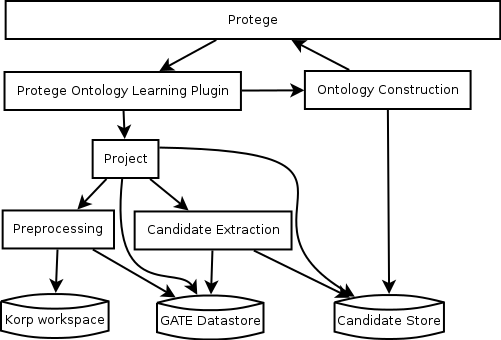
\includegraphics[width=10cm]{graphics/protege-plugin-components-simple.png}
  \caption{Prototype design}
  \label{fig:prototype-design}
\end{figure}

Designed as a plugin to the Protege ontology editor, it can be embedded inside the Protege editor window alongside other plugins designed to ease ontology development and maintenance.
The plugin consists of Protege integration, a graphical user interface and an ontology learning project instance.
The project is used to trigger preprocessing and extraction, and hold references to storage of the corpus and ontology element candidates. After candidate extraction, the Ontology Construction component is used to model the domain in the current OWL ontology in Protege. The project can also be used to extract candidates for use outside of this system.

\begin{figure}
  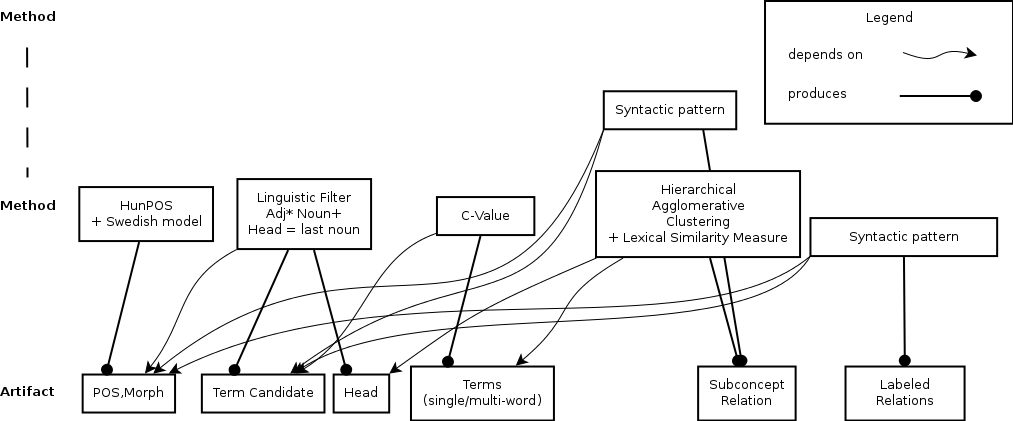
\includegraphics[width=\textwidth]{graphics/method-element-dependencies.png}
  \caption{Methods and artifacts of the prototype}
  \label{fig:method-artifact}
\end{figure}

\subsection{Preprocessing}
% Remember if we want more detail, look back in git.
Preprocessing is done partly using the Korp corpus import pipeline, and partly using GATE.
When a project is created, the corpus can be imported using a filter or simply all files in a given folder.
This adds the documents to a GATE corpus, which extracts the text from various document formats.
For syntactic annotation, the corpus is exported to a directory where the Korp pipeline can take it as input.
The Korp pipeline was configured to annotate the corpus with part of speech tags, lemmas, word boundaries, sentence boundaries, and syntactic dependencies.
When the Korp pipeline finishes processing the corpus, the annotations are imported to the working GATE corpus.
Next, the JAPE rules are run to apply higher-level annotations to the corpus.
The term candidate JAPE rule is described in the next section, while the labeled relation JAPE rule is discussed in Section~\ref{sec:results:proto:cands}.

\subsubsection{Linguistic Filter for Term Candidates}
\label{sec:results:proto:prepr}

For initial potential terms to be selected by the C-Value method, a linguistic filter of zero or more adjectives, followed by one or more nouns, is used.
This filter was depicted as Adj*Noun+ in \cite{Frantzi98CNCValue} by analogy to regular expressions over parts of speech.
The head of these simplistic noun phrases was selected as the last noun in the phrase, as is common with this form of noun phrases.
I refer to the noun phrases that were selected as potential terms as \emph{term candidates} and they are used in term extraction, subconcept relation extraction and labeled relaton extraction.

I initially experimented with noun phrases extracted using the SweSPARK noun phrase chunker, but the Adj*Noun+ form of noun phrase was most-suited to the similarity measure for Hirarchical Agglomerative Clustering.
The chunker provides many forms of noun phrases including determiners and other parts of speech which are not clearly part of terms.
Selecting the head noun in certain noun phrase forms such as DetAdj*Noun+PrepNoun is more complex than for Adj*Noun+ phrases, and the similarity measure used in \cite{Drymonas10OntoGain} needs to have the head identified.
The Adj*Noun+ form performed well for English in the evaluation of C-Value in \cite{Frantzi98CNCValue} and many Swedish noun phrases take this form \todo{cite swedish noun phrase book} so this was a reasonable approximation for the objective of this thesis.
For better results, more experimentation is needed to identify more effective linguistic filters for Swedish, but as with all patterns and models, the ideal can vary between domains and corpora.

The initial term candidate selection was performed as annotations in the corpus along with syntactic feature annotation for convenience.
This was performed using JAPE expressions matching on parts of speech annotations in the corpus.
This implementation made it easy to implement and verify that it is working as intended.
The JAPE expression is written in a plain text file which can easily be modified to experiment with different patterns, and separates the concerns of the Java code controlling the entire tool and the linguistic filter itself.
The JAPE expression defining the filter is shown in Listing~\ref{lst:termcand}.

\begin{Code}
\lstset{caption={JAPE for term candidate linguistic filter},
           captionpos=b,
           label={lst:termcand}
}
\begin{lstlisting}[frame=single]
(
  ({w.pos == "JJ"})*
  ({w.pos == "NN"}|{w.pos == "PM"})+
): match
-->
:match.TermCandidate = {rule= "LingFilter" }
\end{lstlisting}
\end{Code}

\subsection{Candidate Extraction}

For each of the typical layers of ontologies, one or two types of element were extracted to demonstrate some relevant method.
Methods with an important linguistic component are the most interesting in this case. 
For concepts, labeled concepts were extracted.
For taxonomic relations, subconcept relations were extracted.
For non-taxonomic relations, labeled relations between concepts were extracted.

\subsubsection{Concepts}

Concepts are assumed to be represented by terms in the corpus.
Term candidates are extracted using the C-value part from the C-value NC-value method for extracting multi-word terms.
The C-value method is applied to the strings annotated with the TermCandidate annotation as described in Section~\ref{sec:results:proto:prepr}.
The C-value is always a product of \(log_{2} |a|\) where \(a\) is the candidate string and \(|a|\) is the number of words in the string.
For single-word terms, C-value would normally be \(0\).
To be able to use C-value as a relevance measure for single- and multi-word terms, we calculate C-value as a product of \(log_{2} (|a|+1)\) instead.
Single-word terms are thus given useful C-values, instead of being totally disregarded.
The modified C-value is referred to as \emph{confidence}, representing the confidence that a given term is relevant to the domain being modeled.

\subsubsection{Subconcept Relations}

Two methods for extracting subclass relations were implemented.
One method uses hierarchical agglomerative clustering, and the other uses a syntactic pattern.

The hierarchical agglomerative clustering method used takes term candidates as input and creates subclass relations from one term candidate to another.
The similarity measure is that used in~\cite{Drymonas10OntoGain}.
Merging for a given cluster stops when no other cluster has a common noun phrase head.
The noun phrase head is taken as the superconcept of all terms in the cluster.
Thus a subclass relation candidate is created between each term and its noun phrase head.
This method is only used on the 1000 term candidates with highest confidence since the implementation has time complexity of \(\mathcal{O}(n^{3})\).

The syntactic pattern method used a translation of one pattern used in Text2Onto\cite{Cimiano2005Text2Onto}.
The pattern \(NP such as (NP, |NP and)* NP\) has been implemented with \emph{such as} replaced with \emph{såsom} as shown in Listing~\ref{lst:saasom}.
The JAPE code before the \verb+-->+ works like a regular expression on annotations.
The regular expression tries to match one TermCandidate annotation, followed by zero or more commas, then the string "såsom", followed by one or more TermCandidate annotations separated by comma, "och" or "eller".
Each time this regular expression matches, the part after the \verb+-->+ adds new annotations.
The first matching term candidate is annotated with "Range".
The subsequent term candidates are annoted with "Domain".
The entire matching region is annotated with "SubclassOf".
This JAPE rule is executed during preprocessing after the other JAPE rules for convenience.
During extraction, we iterate over all SubclassOf annotations, adding a subclass relation to the term annotated with Range for each term candidate in the contained Domain annotation.

\begin{Code}
\lstset{caption={JAPE for subclass relation annotations by syntactic pattern},
           captionpos=b,
           label={lst:saasom}
}
\begin{lstlisting}[frame=single]
(
	({TermCandidate}):superconcept
	({w.string==","})?
	{w.string=="såsom"}
	({TermCandidate}
	  ({w.string==","}
	   |{w.string=="och"}
	   |{w.string=="eller"})?)+
	    :subconcept
):subclassOf
-->
:subclassOf.SubclassOf = { rule = "SubclassOfRelation1" },
:subconcept.Domain     = { rule = "SubclassOfRelation1" },
:superconcept.Range    = { rule = "SubclassOfRelation1" }
\end{lstlisting}
\end{Code}

\subsubsection{Labeled relations}
\label{sec:results:proto:cands}

Labeled relation extraction was based on syntactic dependency relations - one per sentence - where the appropriate annotations are found.
The domain of the relation is the term candidate with a subject relation (SS) to the root.
The range of the relation is the term candidate with an object relation (OO) to the root.
The label of the relation is dependency root of the sentence, if it is a verb (VB), potentially followed by an additional verb which has a verb group relation (VG) to the root if one exists.

To ease the task of selecting relevant candidates to be used in constructing the ontology, an \emph{importance} value is calculated for each labeled relation candidate.
This value is intended to indicate importance to the domain being modeled.
The value is calculated as the sum of the confidence of the domain and range term candidates for each occurrence of the relation.
Relations between important term candidates are thus favoured, as are frequently-occurring relations.

\subsection{Ontology Construction}

The Ontology Construction component is responsible for modelling the domain in an OWL ontology based on the extracted ontology element candidates.
The user can either add all candidates to the ontology in one step, or select specific candidates and add only them to the ontology.

Concept candidates are added as OWL Classes.
The IRI of a class is constructed as the concept label in camel case appended to the ontology IRI.
Thus a term "akut hjärtinfarkt" could be a class with the IRI fragment as \#AkutHjärtinfarkt.

Subconcept relations are modeled as RDFS subClassOf relations.
This implies that all properties of the superclass are also properties of its subclasses.

Labeled relations are modeled using OWL Object Properties.
For a relation \(r\) from concept \(a\) to concept \(b\), we express in OWL that \(a\) is a subclass of an anonymous class whose instances have a relation \(r\) to at least one instance of \(b\).
This does not imply that all instances which have relation \(r\) to an instance of \(b\) are instances of \(a\).
It only expresses that it is necessary to have a relation \(r\) to an instance of \(b\) to be an instance of \(a\).
This way of modelling the relation ers on the side of making a weak assertion but remaining correct until more information is available.
An alternative way to model these relations would be to create an anonymous class for the domain and range of each relation, where the anonymous class is the union of all classes which are in the subject or object position of that relation, respectively.
That way of modelling it would incorrectly classify any instance with that relation as one of the classes in the union, until that instance's superclass is discovered and added to the union.
The chosen modelling approach is not always appropriate and more options are needed here.

\section{Ontology learning evaluation}
\label{sec:results:eval}

\chapter{Analysis}
\label{chapter:analysis}

\section{Implementation}

%%UU-REQ Evidence that the student has made a critical evaluation of the significance of the project outcomes, limitations of the results
%UU-CHAP Data collection and analysis where relevant, or testing of the solution of product.
%% Critical analysis of the results - show you know its limitations

\subsection{Preprocessing}

I should probably have assumed nicely-formatted input rather than being concerned with handling any bunch of PDFs or whatever.
Handling all sorts of input, a bit like T2O, is a nice idea for a real life OL system but given that my objective is to focus on learning about OL from Swedish, preprocessing crap was out of scope. 
\todo{obviously make this more formal and structured, but then also add references to the part of the analysis where I identify bad results due to formatting and unclean input.}

Informally, I didn't use SVENSK because it was difficult to find\footnote{try googling SVENSK language processing, and the URL in \cite{Olsson98SVENSKTagging} is broken, I only just found the old site in the internet archive wayback machine}, I don't think it was mentioned in the BLARK report\todo{check}, and more recent language processing tools existed than those included in SVENSK and better performance from these could be expected.
However, I could have learnt something useful by looking at their lessons learnt.
They also used GATE and talk a lot about what they learnt in trying to make a general purpose language processing tool.
Keeping the preprocessing general in an OL system would probably help in supporting pluggable IE components and might support related research or benefit from easy integration of new preprocessing tools. \todo{formalize this para}


\chapter{Conclusion}
%%UU-CHAP Conclusions reached and future enhancement or work that could be conducted to refine the system.
%%UU-REQ Strength of the conclusions reached, including the ability to provide a concise summary of the significance of the work and reflect on work practice and outcomes with the intent to improve performance in future projects.
% summarise introduction with detail from Solution and Evaluation

\section{Further Work}
%% show you know what’s missing

\section{Personal reflections}

If I did it again, I'd start out reading a research guide like Creswell's \cite{creswell2003research}.

The expectations still feel a bit unclear, even though I'm more familiar with the process. It's difficult to bring together the ideas of "master's level doesn't need original reseach", "it's not a programming exercise", "most people go and program something at a company", the thesis course outcomes and the variety of master's level guides - some universities lean more towards a researchy feel and some more towards a software engineering feel. Not to mention the variety in quality and researchyness of reports in Uppsala's DiVA archives. I think the issue about original research comes from the requirement that we must "delimit a scientific problem" ... and once you involve science you involve research methods, which involve novelty for relevance. If this is correct and this rule can be broken, it should be clearer how to break it without breaking some other rule you're not allowed to break.

\todo{check if a section such as this is expected, required, and what is expected of it.}

\clearpage
%\addcontentsline{toc}{chapter}{References}
%\renewcommand\bibname{References}

%\renewcommand{\refname}{}
%\chapter{References}
\bibliographystyle{unsrt}
\bibliography{report}

\end{document}
